\subsection{Телескоп}
\term{Телескоп}~--- устройство для наблюдения удаленных объектов. На данный момент существуют телескопы  для наблюдения во всех  диапазонах электро-магнитного излучения. По наблюдаемому диапазону телескопы делят на \imp{оптические} телескопы, \imp{радиотелескопы}, \imp{рентгеновские} телескопы и \imp{гамма-те\-ле\-скопы}. Каждый из классов в свою очередь содержит множество подклассов. Поговорим подробнее про оптические телескопы.

Оптические телескопы по своей схеме делятся на три типа: \imp{рефлекторы} (диоптрические), \imp{рефракторы} (катаптрические) и \imp{катадиоптрические}.

%\subsubsection*{Рефрактор} 
Оптический телескоп, в котором для собирания света используется система линз называется \term{рефрактором} (\imp{зеркальным телескопом}). Апертура телескопа определяется диаметром главной линзы. Существует две оптические схемы телескопов-рефракторов. 

\vspace{-.3pc}
\begin{figure}[h!]
	\centering
	\begin{subfigure}{0.49\tw}
		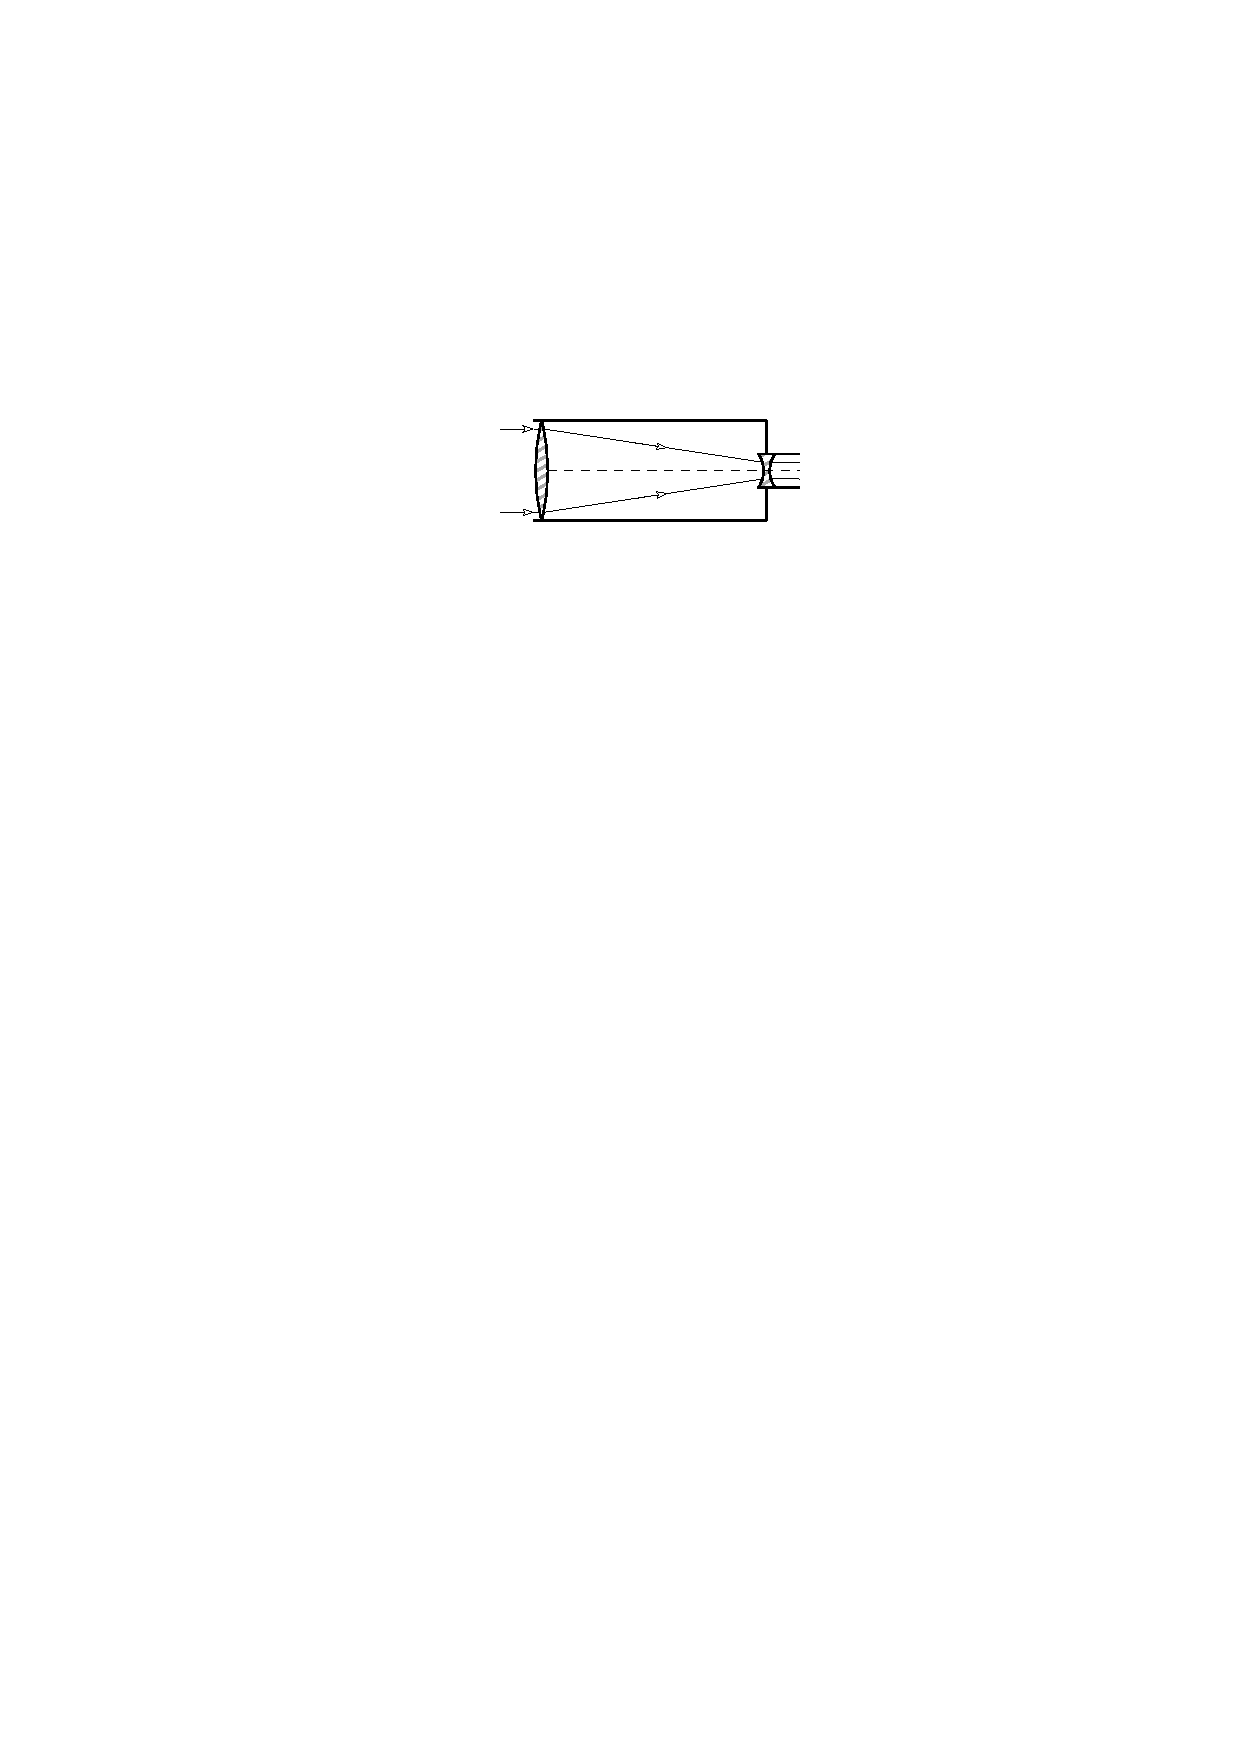
\includegraphics[width = \tw]{Galiley}
		\caption{Рефрактор системы Галилея}
	\end{subfigure}
	\hfill
	\begin{subfigure}{0.49\tw}
		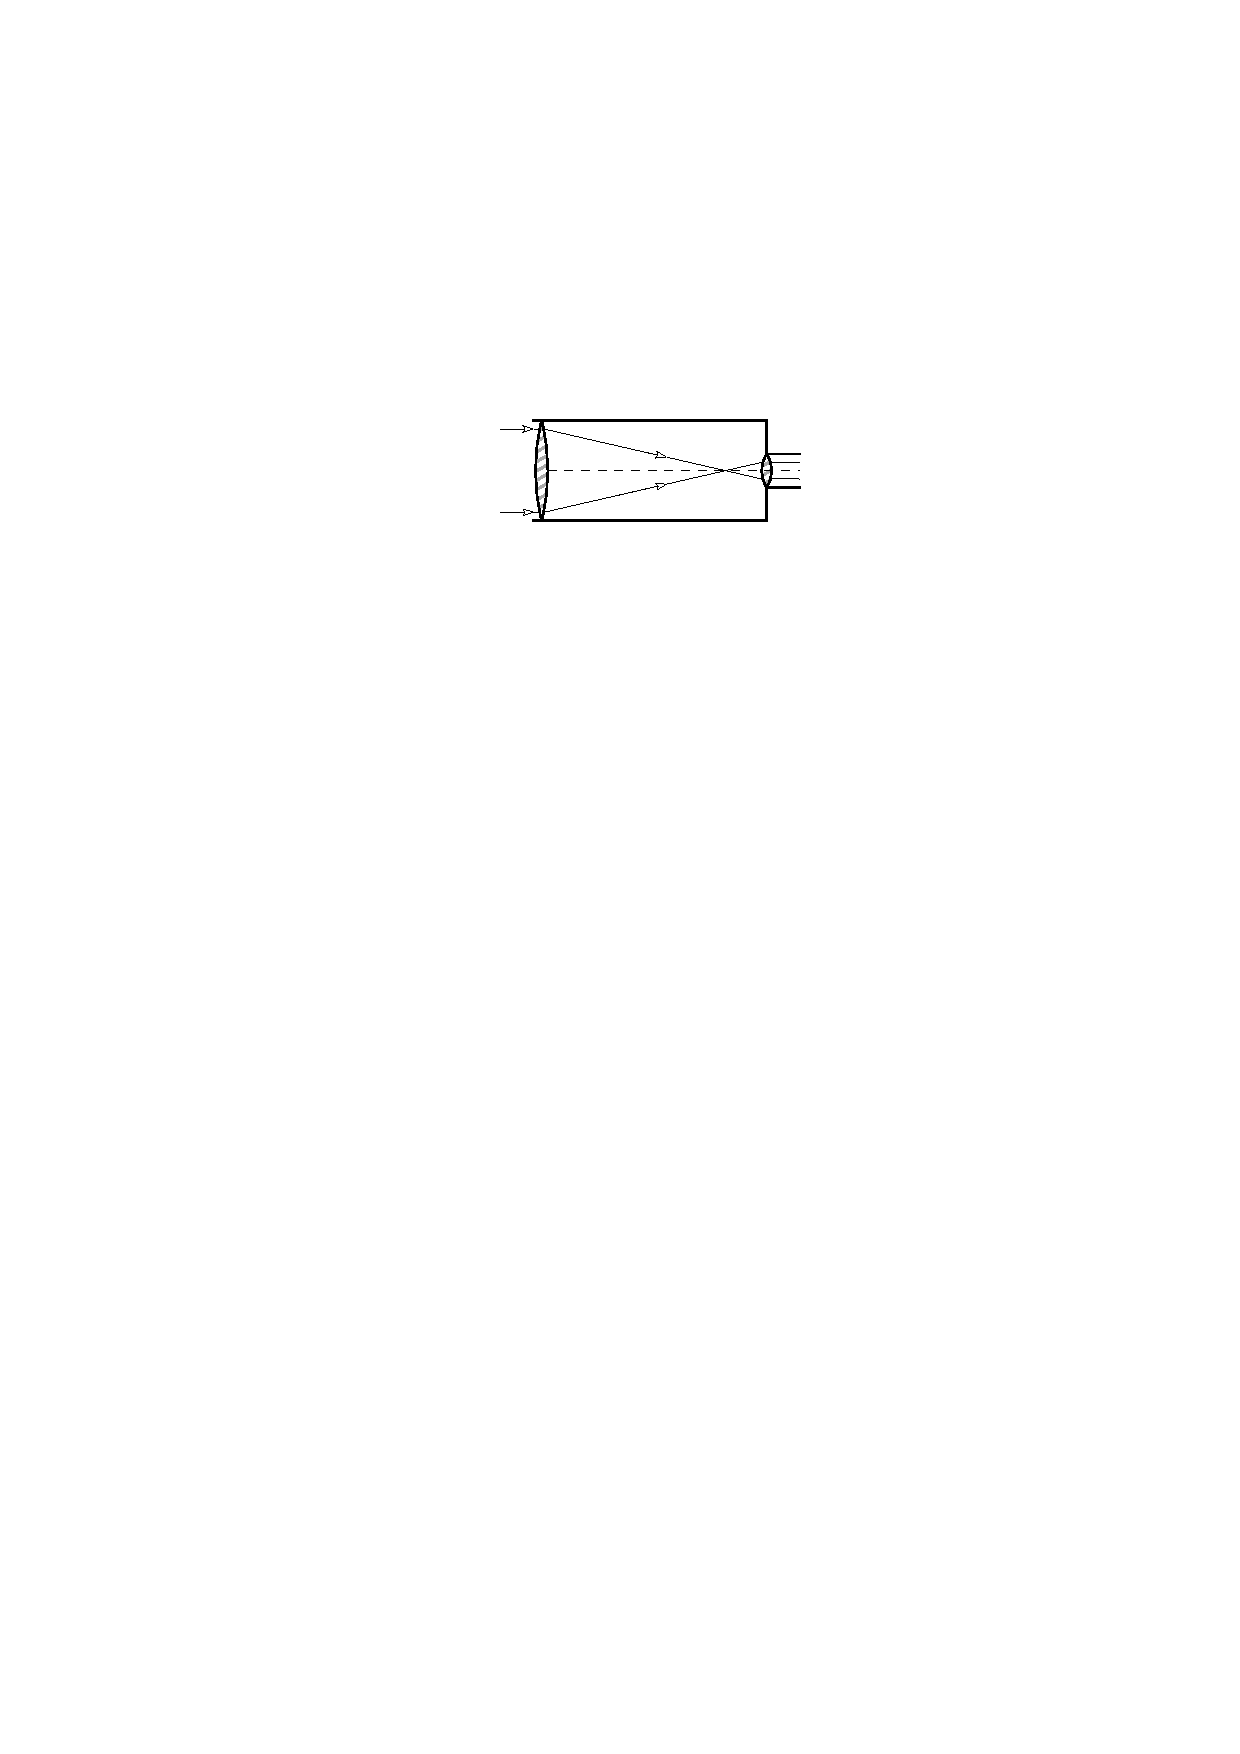
\includegraphics[width = \tw]{Kepler}
		\caption{Рефрактор системы Кеплера}
		\label{Kepler}
	\end{subfigure}
	\caption{Оптические схемы телескопов рефракторов}
\end{figure}

\imp{Система Галилея}~--- окуляр является рассеивающей линзой и располагается перед фокусом главной линзы, изображение прямое. И \imp{система Кеплера}~--- окуляром является положительная (собирающая) линза, находящаяся за главным фокусом, следовательно, телескоп такой схемы дает перевернутое изображение.

%\subsubsection*{Рефлектор} 
Оптический телескоп,  в котором светособирающими элементами являются зеркала называется \term{рефлектором} (\imp{зеркальным телескопом}). Апертура определяется диаметром главного зеркала. В силу удобства изготовления рефлекторов, они пользуются большой попопулярностью за счёт невысокой относительно рефракторов цены. Кроме того использование зеркал в оптической схеме позволяет сильно её разнообразить. Зеркально-линзовый телескоп называется \term{катадиоптрическим}~--- телескоп, в котором используется как система линз, так и зеркал. В обиходе часто не различают рефлекторы и катадиоптрики, обращая внимание лишь на тип главного собирающего элемента. 

\vspace{-.3pc}
\begin{figure}[h!]
	\begin{subfigure}{0.49\tw}
		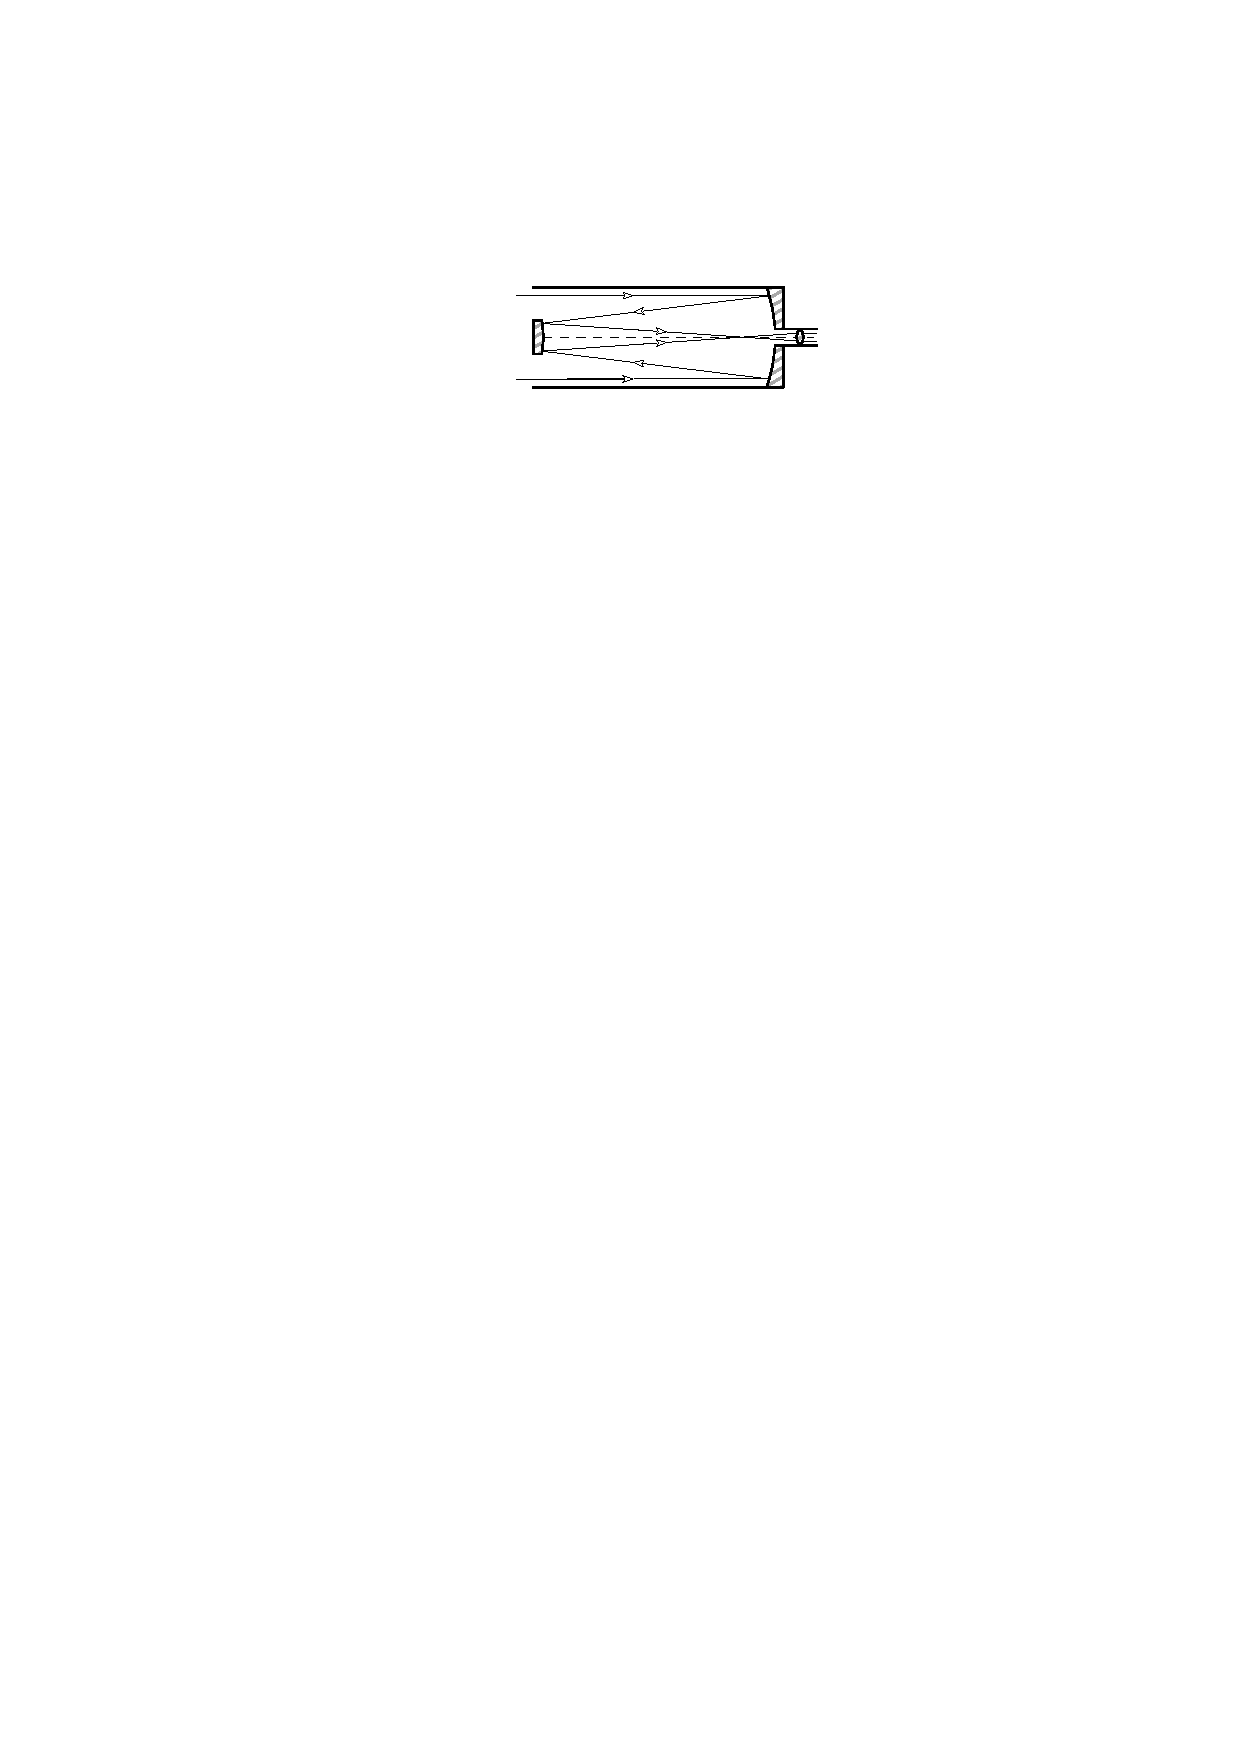
\includegraphics[width = \tw]{Cassigren.pdf}
		\caption{Рефлектор системы Кассегрена}
	\end{subfigure}
	\hfill
	\begin{subfigure}{0.49\tw}
		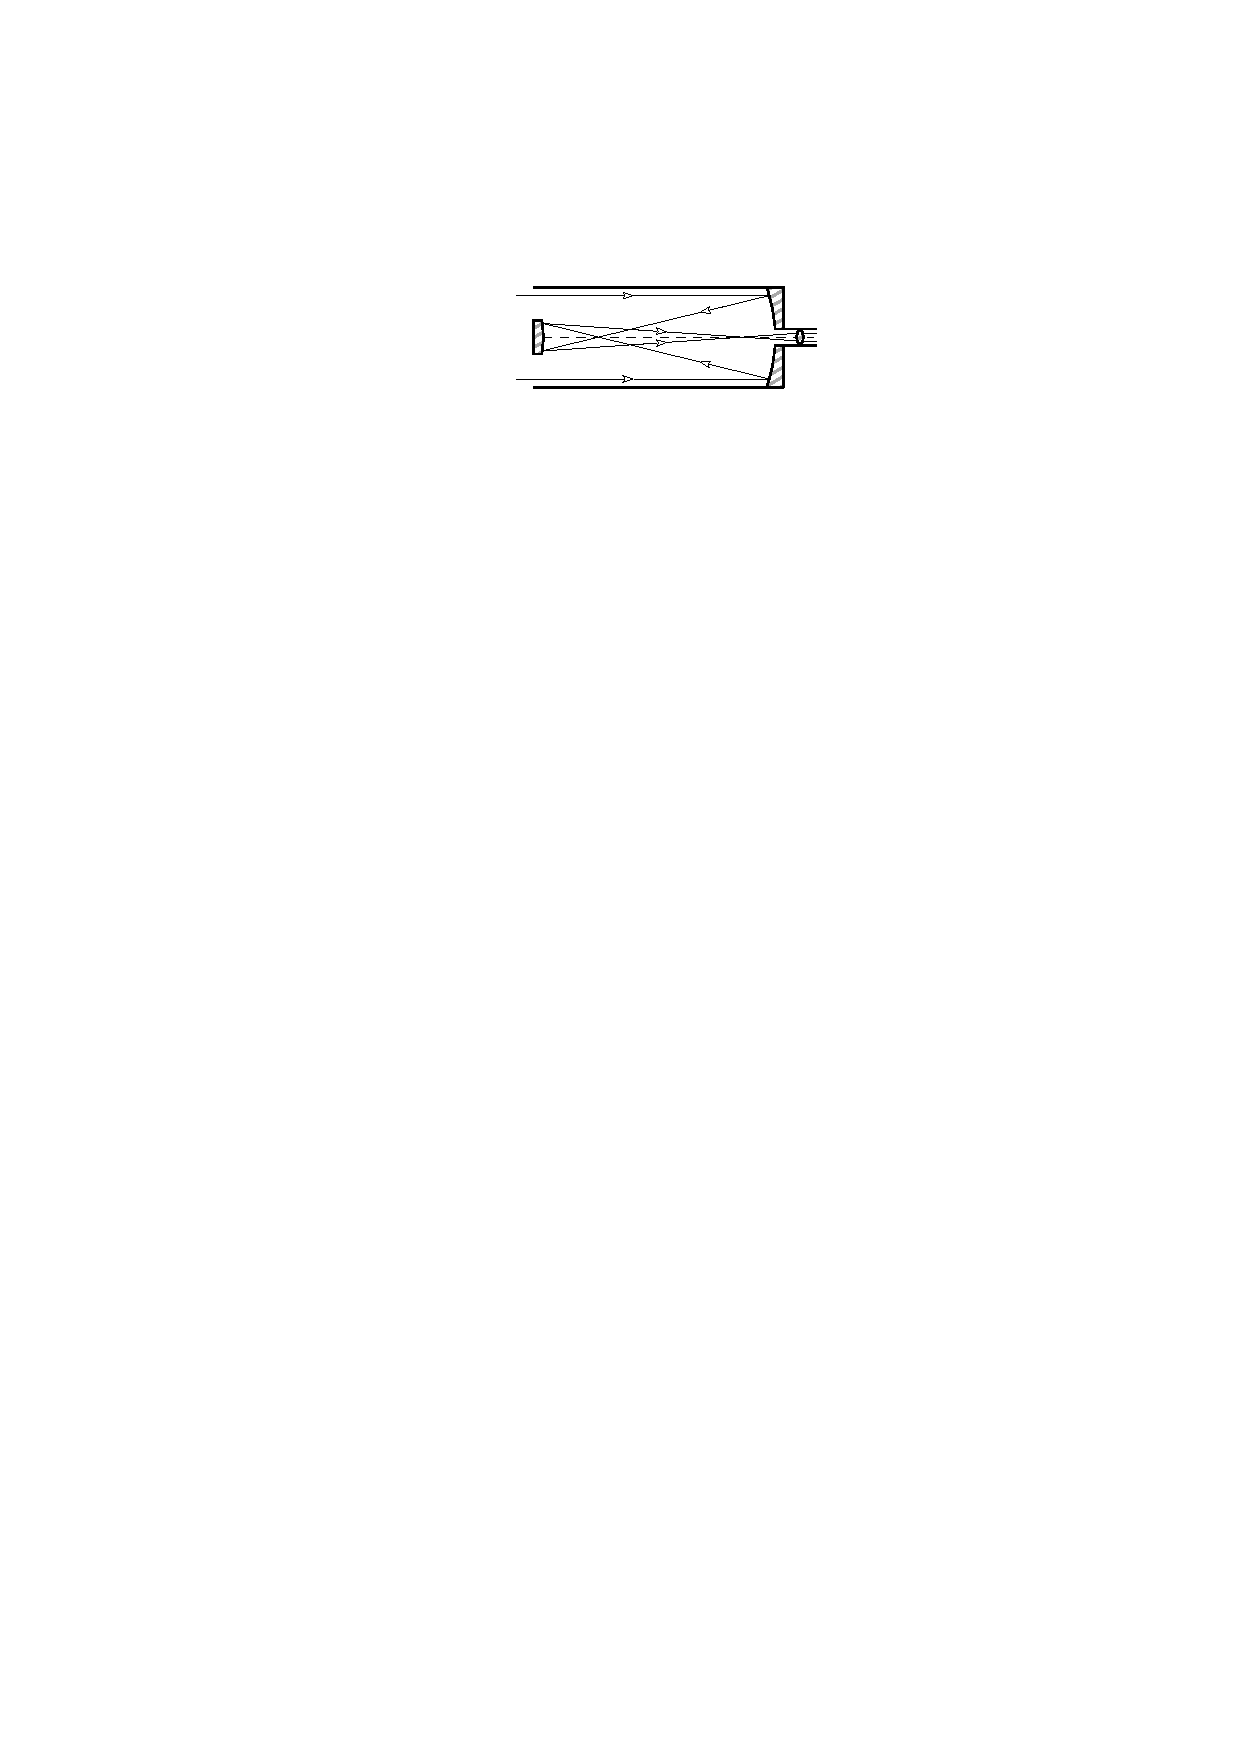
\includegraphics[width = \tw]{Gregory.pdf}
		\caption{Рефлектор системы Грегори}
		\label{Gregory}
	\end{subfigure}
	\vskip4pt
	\begin{subfigure}{0.49\tw}
		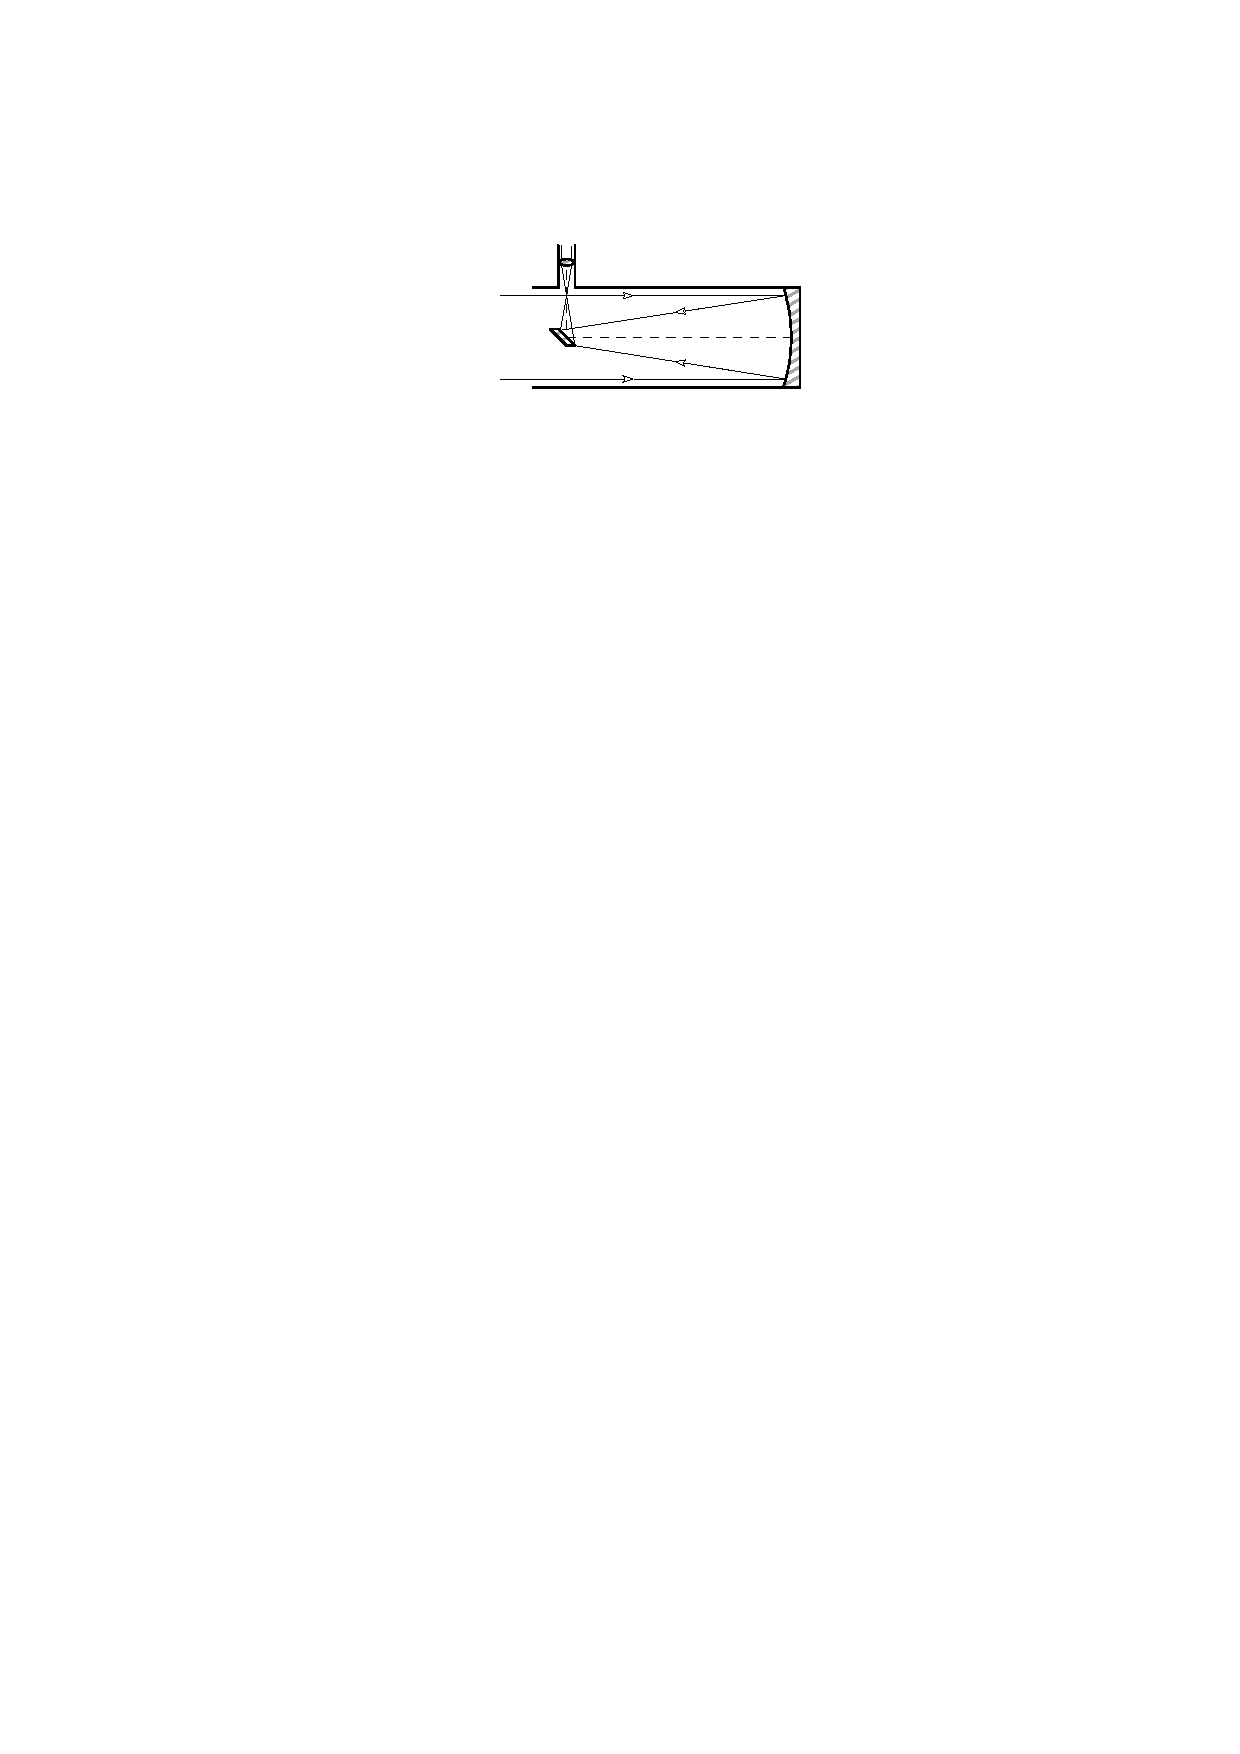
\includegraphics[width = \tw]{Newton}
		\caption{Рефлектор системы Ньютона}
	\end{subfigure}
	\hfill
	\begin{subfigure}{0.49\tw}
		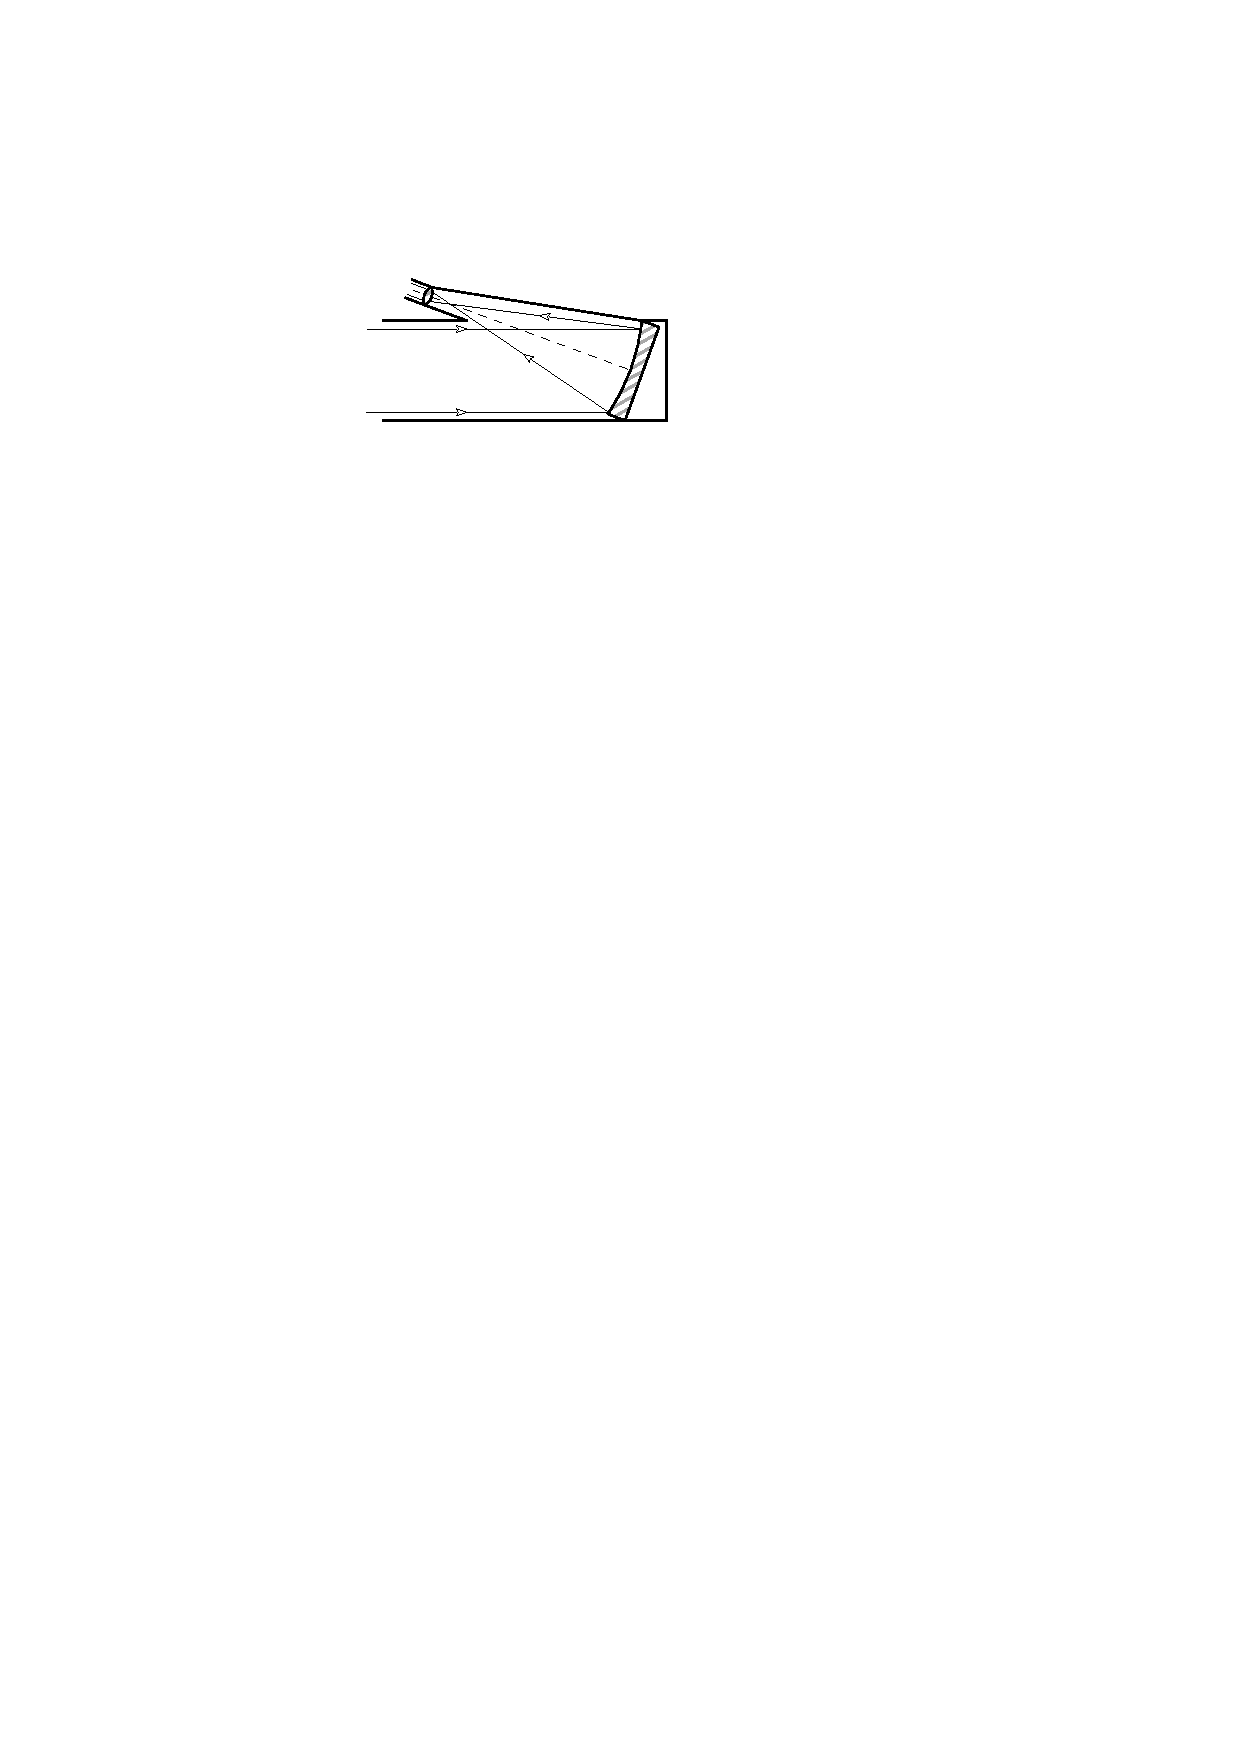
\includegraphics[width = \tw]{Lomonosov.pdf}
		\caption{Рефлектор системы Ломоносова}
	\end{subfigure}
	\caption{Оптические схемы телескопов рефлекторов}
\end{figure}

Первый телескоп телескоп-рефлектор был построен Ньютоном по его же схеме в 1668 году. Главное зеркало параболическое, вторичное~--- плоское, наклонено под $45^\circ$ к оптической оси. Вторичное зеркало в схеме Ньютона поворачивает оптическую ось и выносит фокус из трубы. Изображение получается перевернутым, так как окуляр, как и для все телескопов рефлекторов, являясь собирающей линзой, располагается за фокусом.

Несмотря та то, что Ньютон построил первый телескоп-рефлектор, первую схему телескопа предложим не он, а Грегори, и сделал он это в 1663 году. В его схеме все зеркала расположены соосно, главное~--- параболическое, вторичное~--- эллиптическое. Первый главный фокус в системе Грегори расположен до вторичного зеркала, именно это и позволяет использовать эллиптическое зеркало в качестве вторичного. После вторичного зеркала находится второго главный фокус, а значит, телескоп с такой схемой строит прямое изображение.

В 1672 году Кассегрен предложил модификацию системы Грегори. В качестве вторичного зеркала он предложил использовать выпуклое гиперболическое, вместо вогнутого эллиптического, как было в Грегори. Это позволяет избавиться от второго главного фокуса и сократить размер трубы телескопа. А также такое вторичное зеркало приводит к меньшему экранированию главного, что улучшает проницающую способность. В последствие многие ученые модифицировали систему Кассегрена: добавляли различные апертурные корректоры, меняли форму зеркал. Самыми популярными, а потому и известными стали системы Максутова~--~Кассегрена, Шмидта~--~Кассегрена и Ричи~--~Кретьена.

Описанные выше схемы телескопов обладают важным недостатком: вторичное зеркало затеняет центральную область главного зеркала, причём чем больше относительное отверстие, тем больше затеняемая площадь. В 1762 году М.\,В.~Ломоносов реализовал схему телескопа-реф\-лек\-тора без вторичного зеркала. Главное зеркало в его схеме~--- внеосевой параболоид, фокус которого находится за пределами трубы. К сожалению данная оптическая схема не получила распространения из-за сильной комы.


